\sectionframe{Results of my Masters Thesis}
\section{Masters Thesis}

\begin{frame}{Archetypal Model}
    \begin{figure}
        \stackunder[5pt]{
            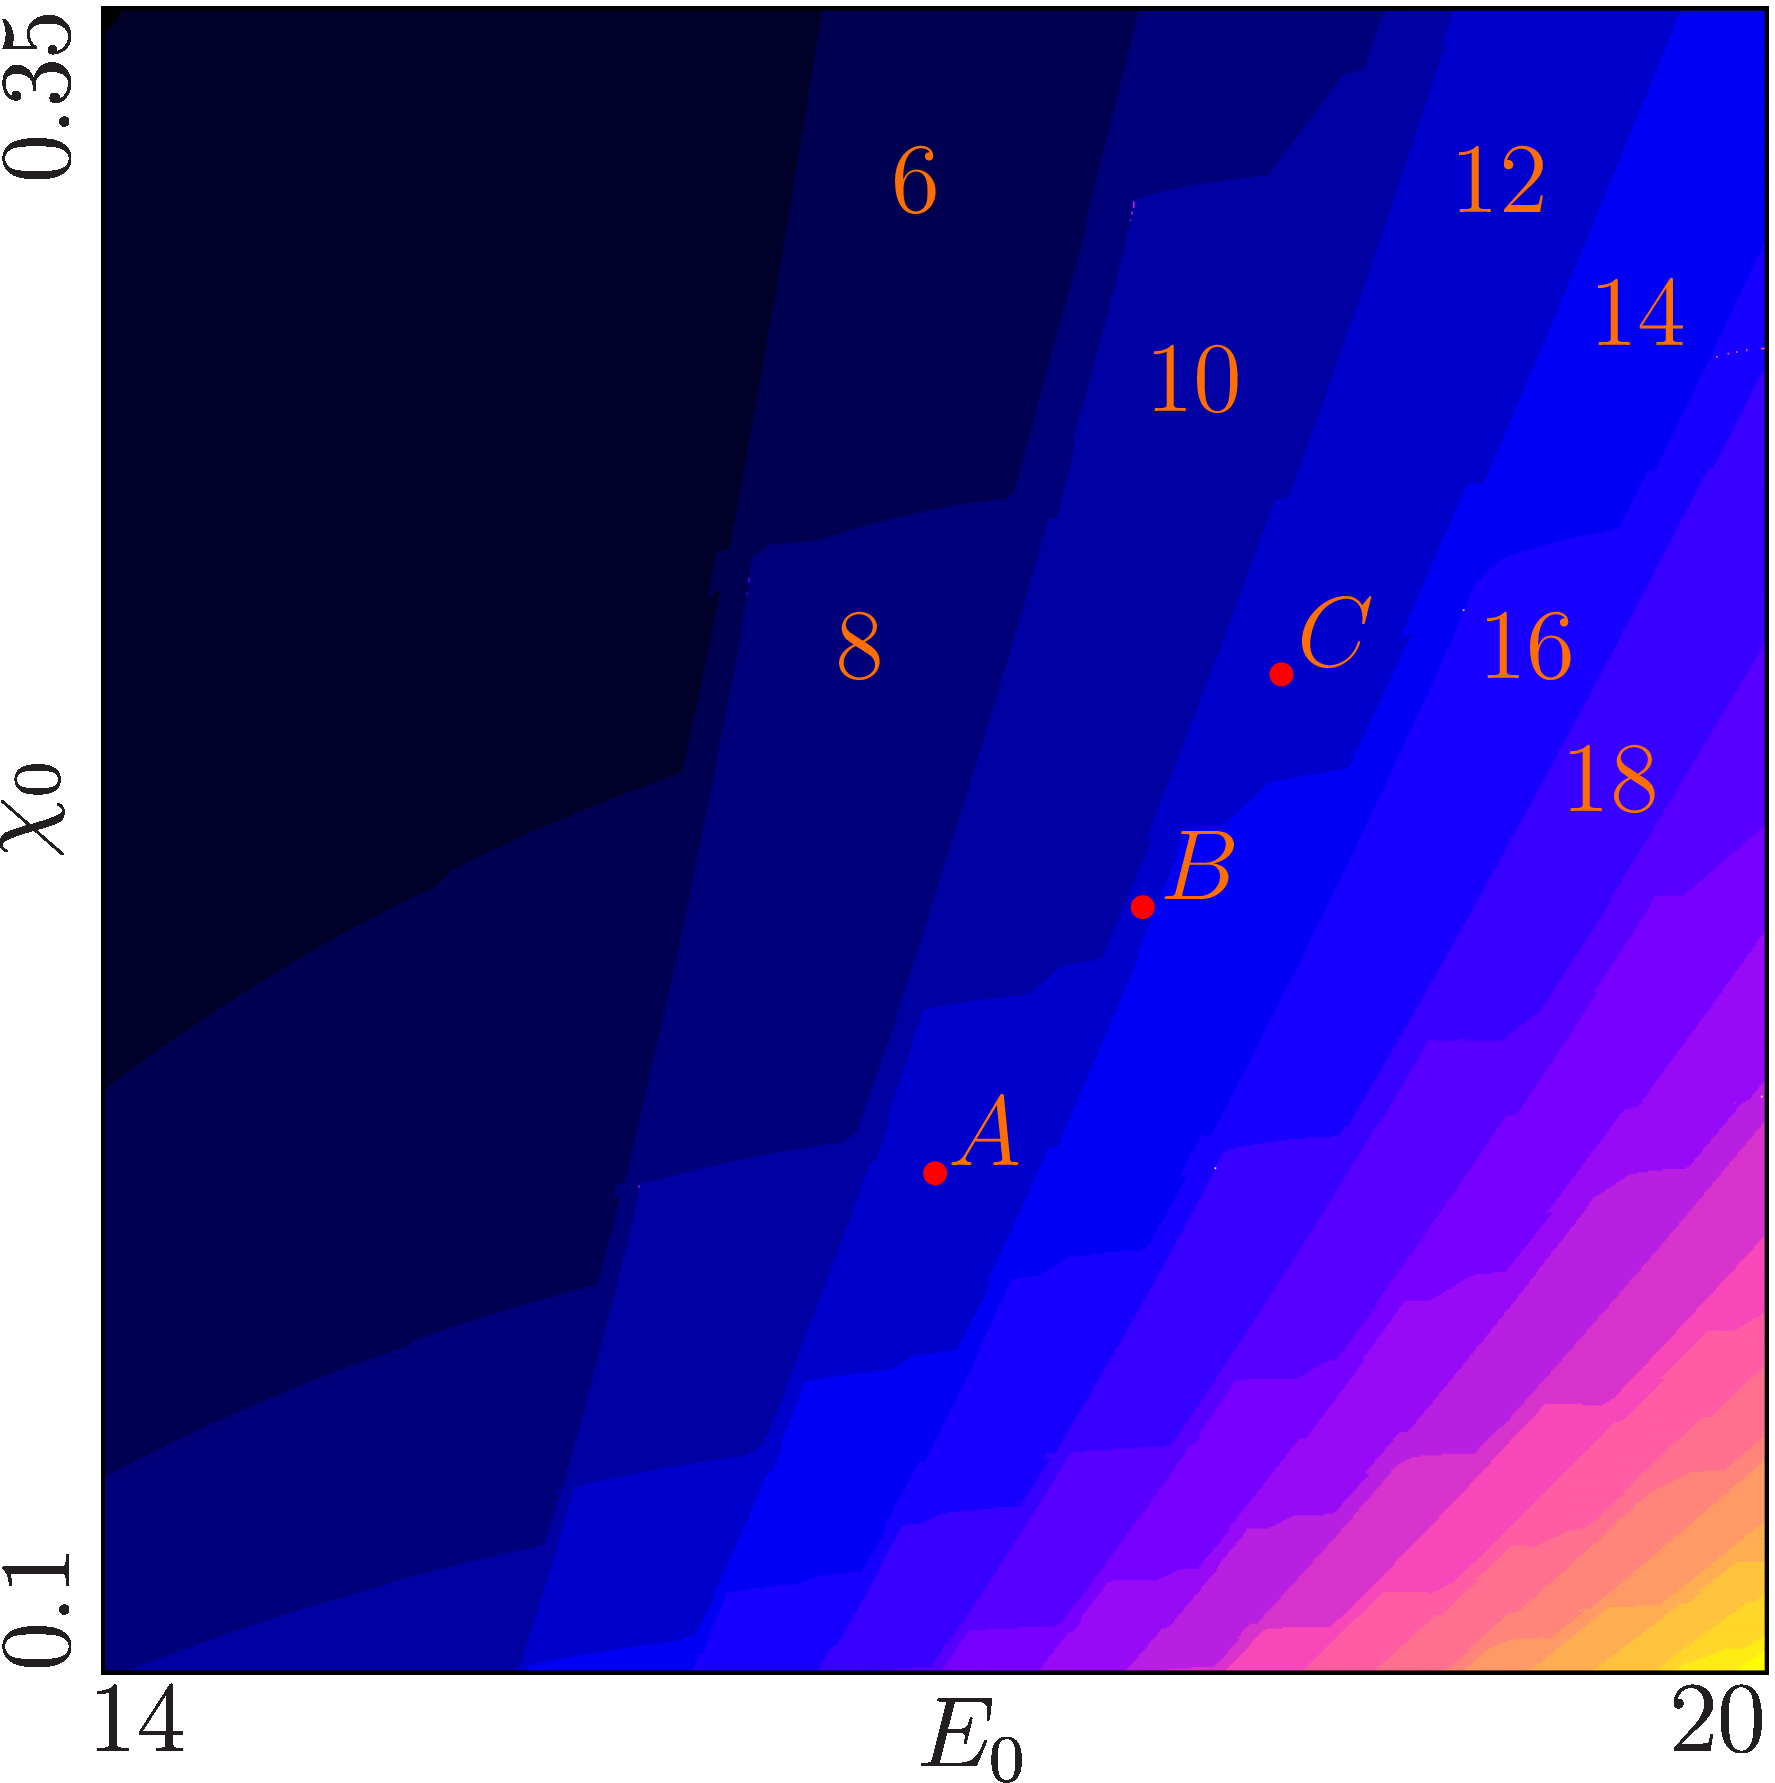
\includegraphics[width=0.4 \textwidth]{Figs/og_model_period.png}
        }{Original model}
        \qquad
        \stackunder[5pt]{
            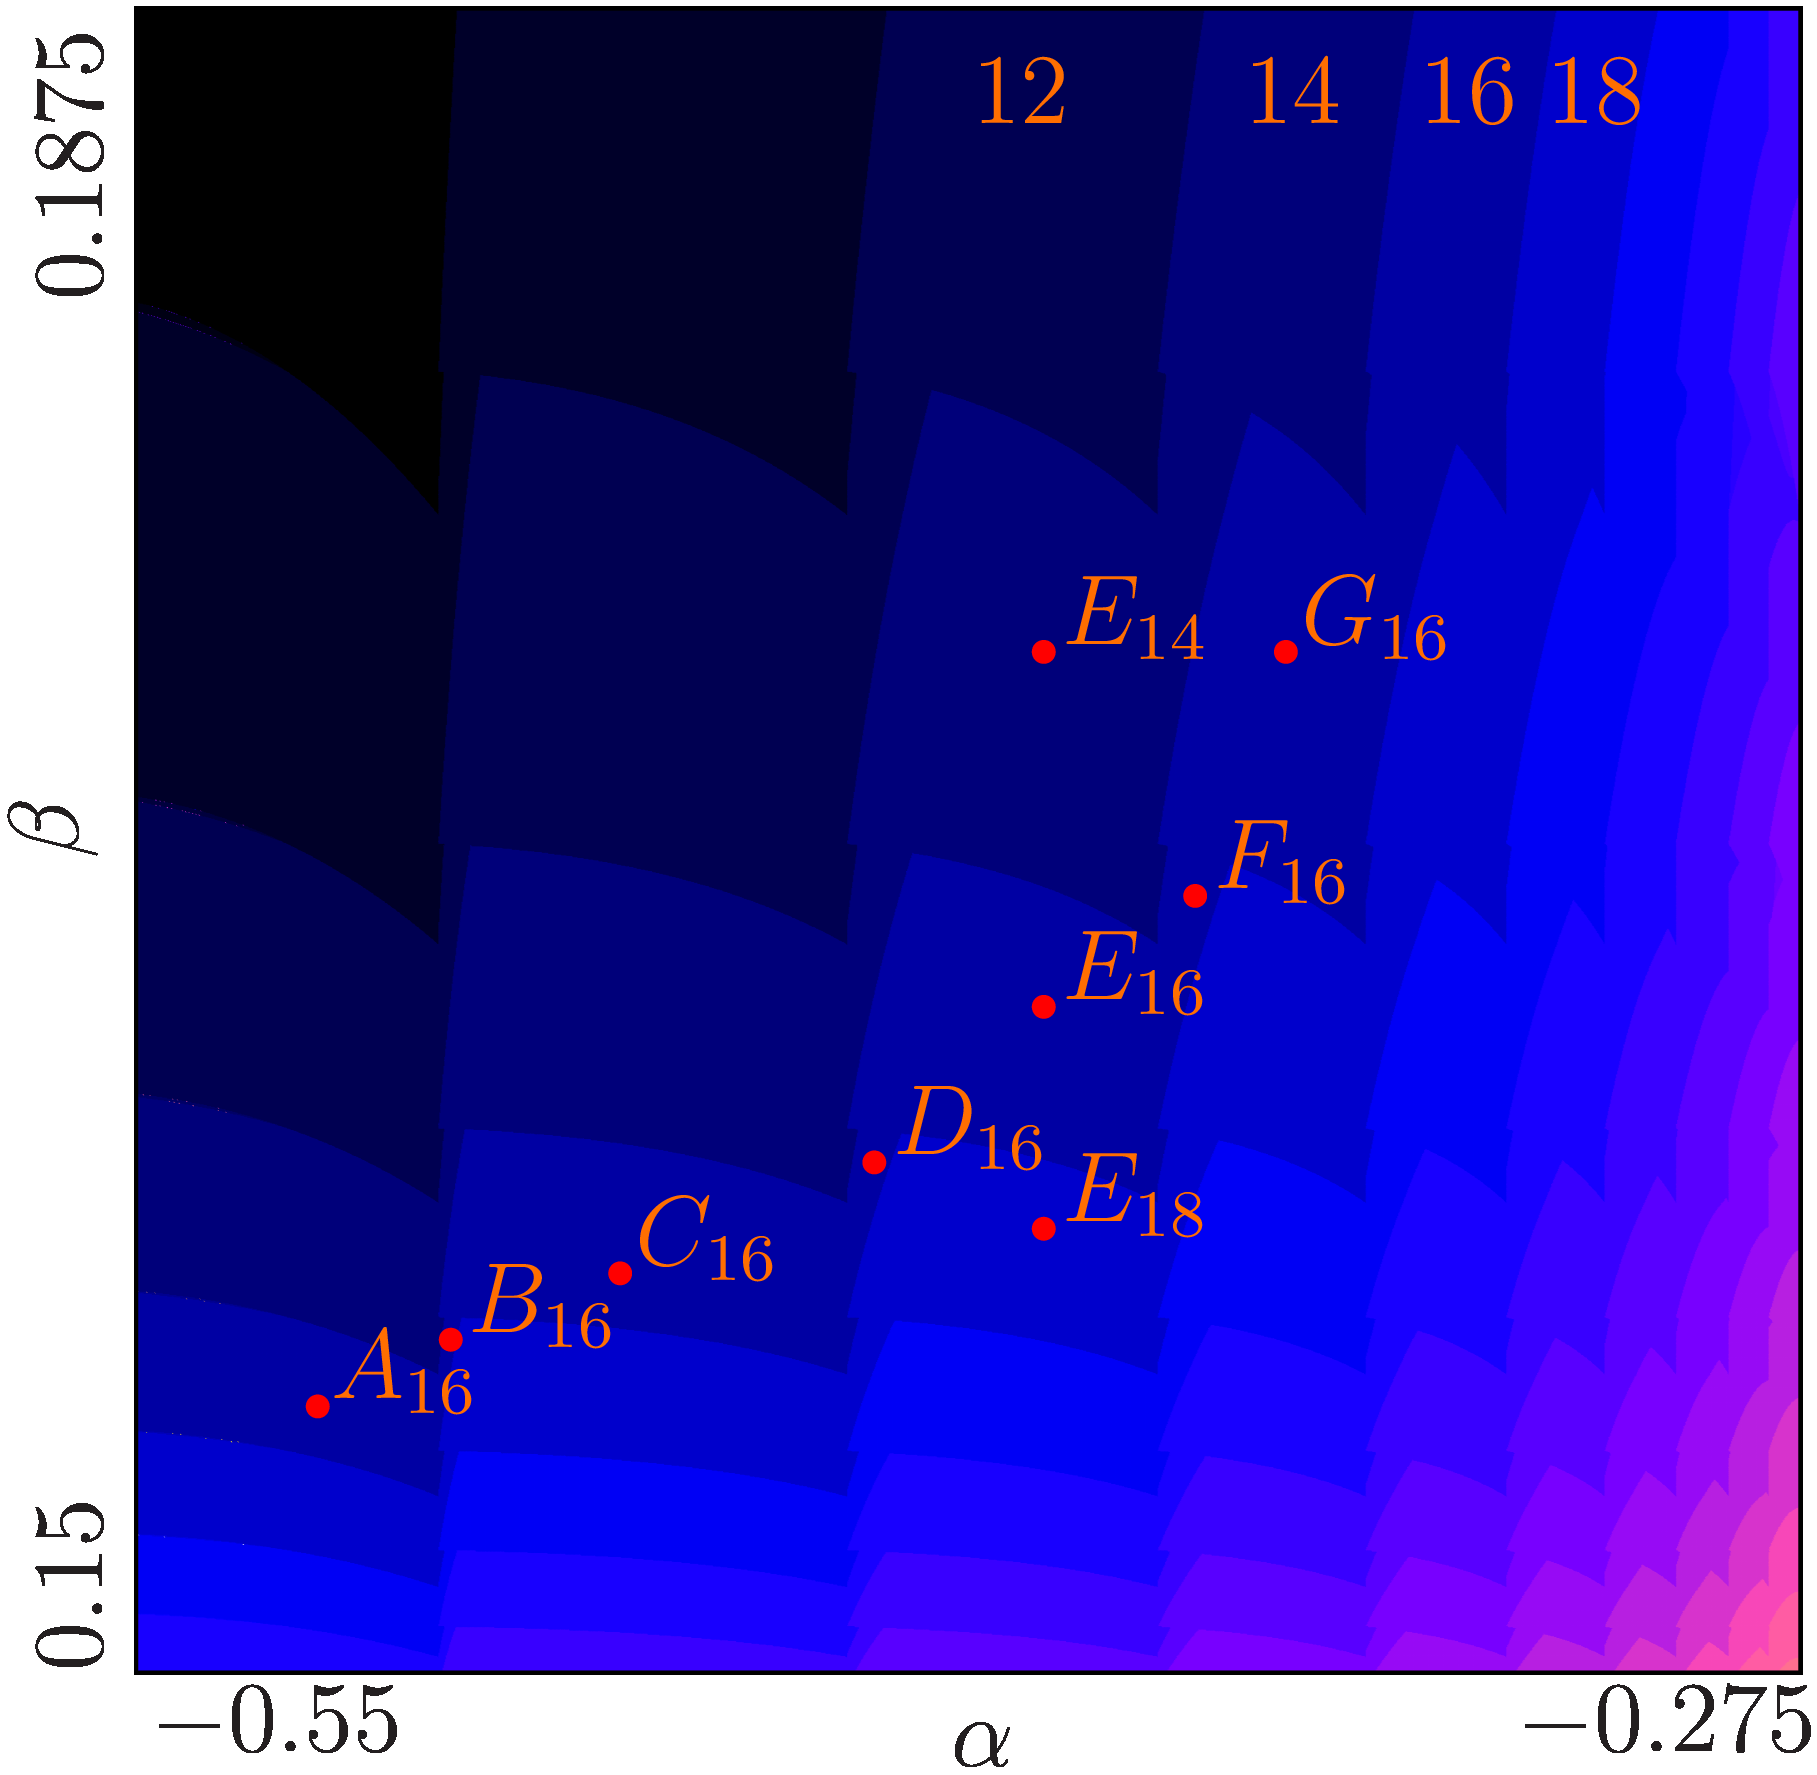
\includegraphics[width=0.41 \textwidth]{Figs/archetypal_model_period.png}
        }{Archetypal model}
    \end{figure}
\end{frame}

\begin{frame}{Archetypal Model}
    \begin{figure}
        \centering
        \stackunder[5pt]{
            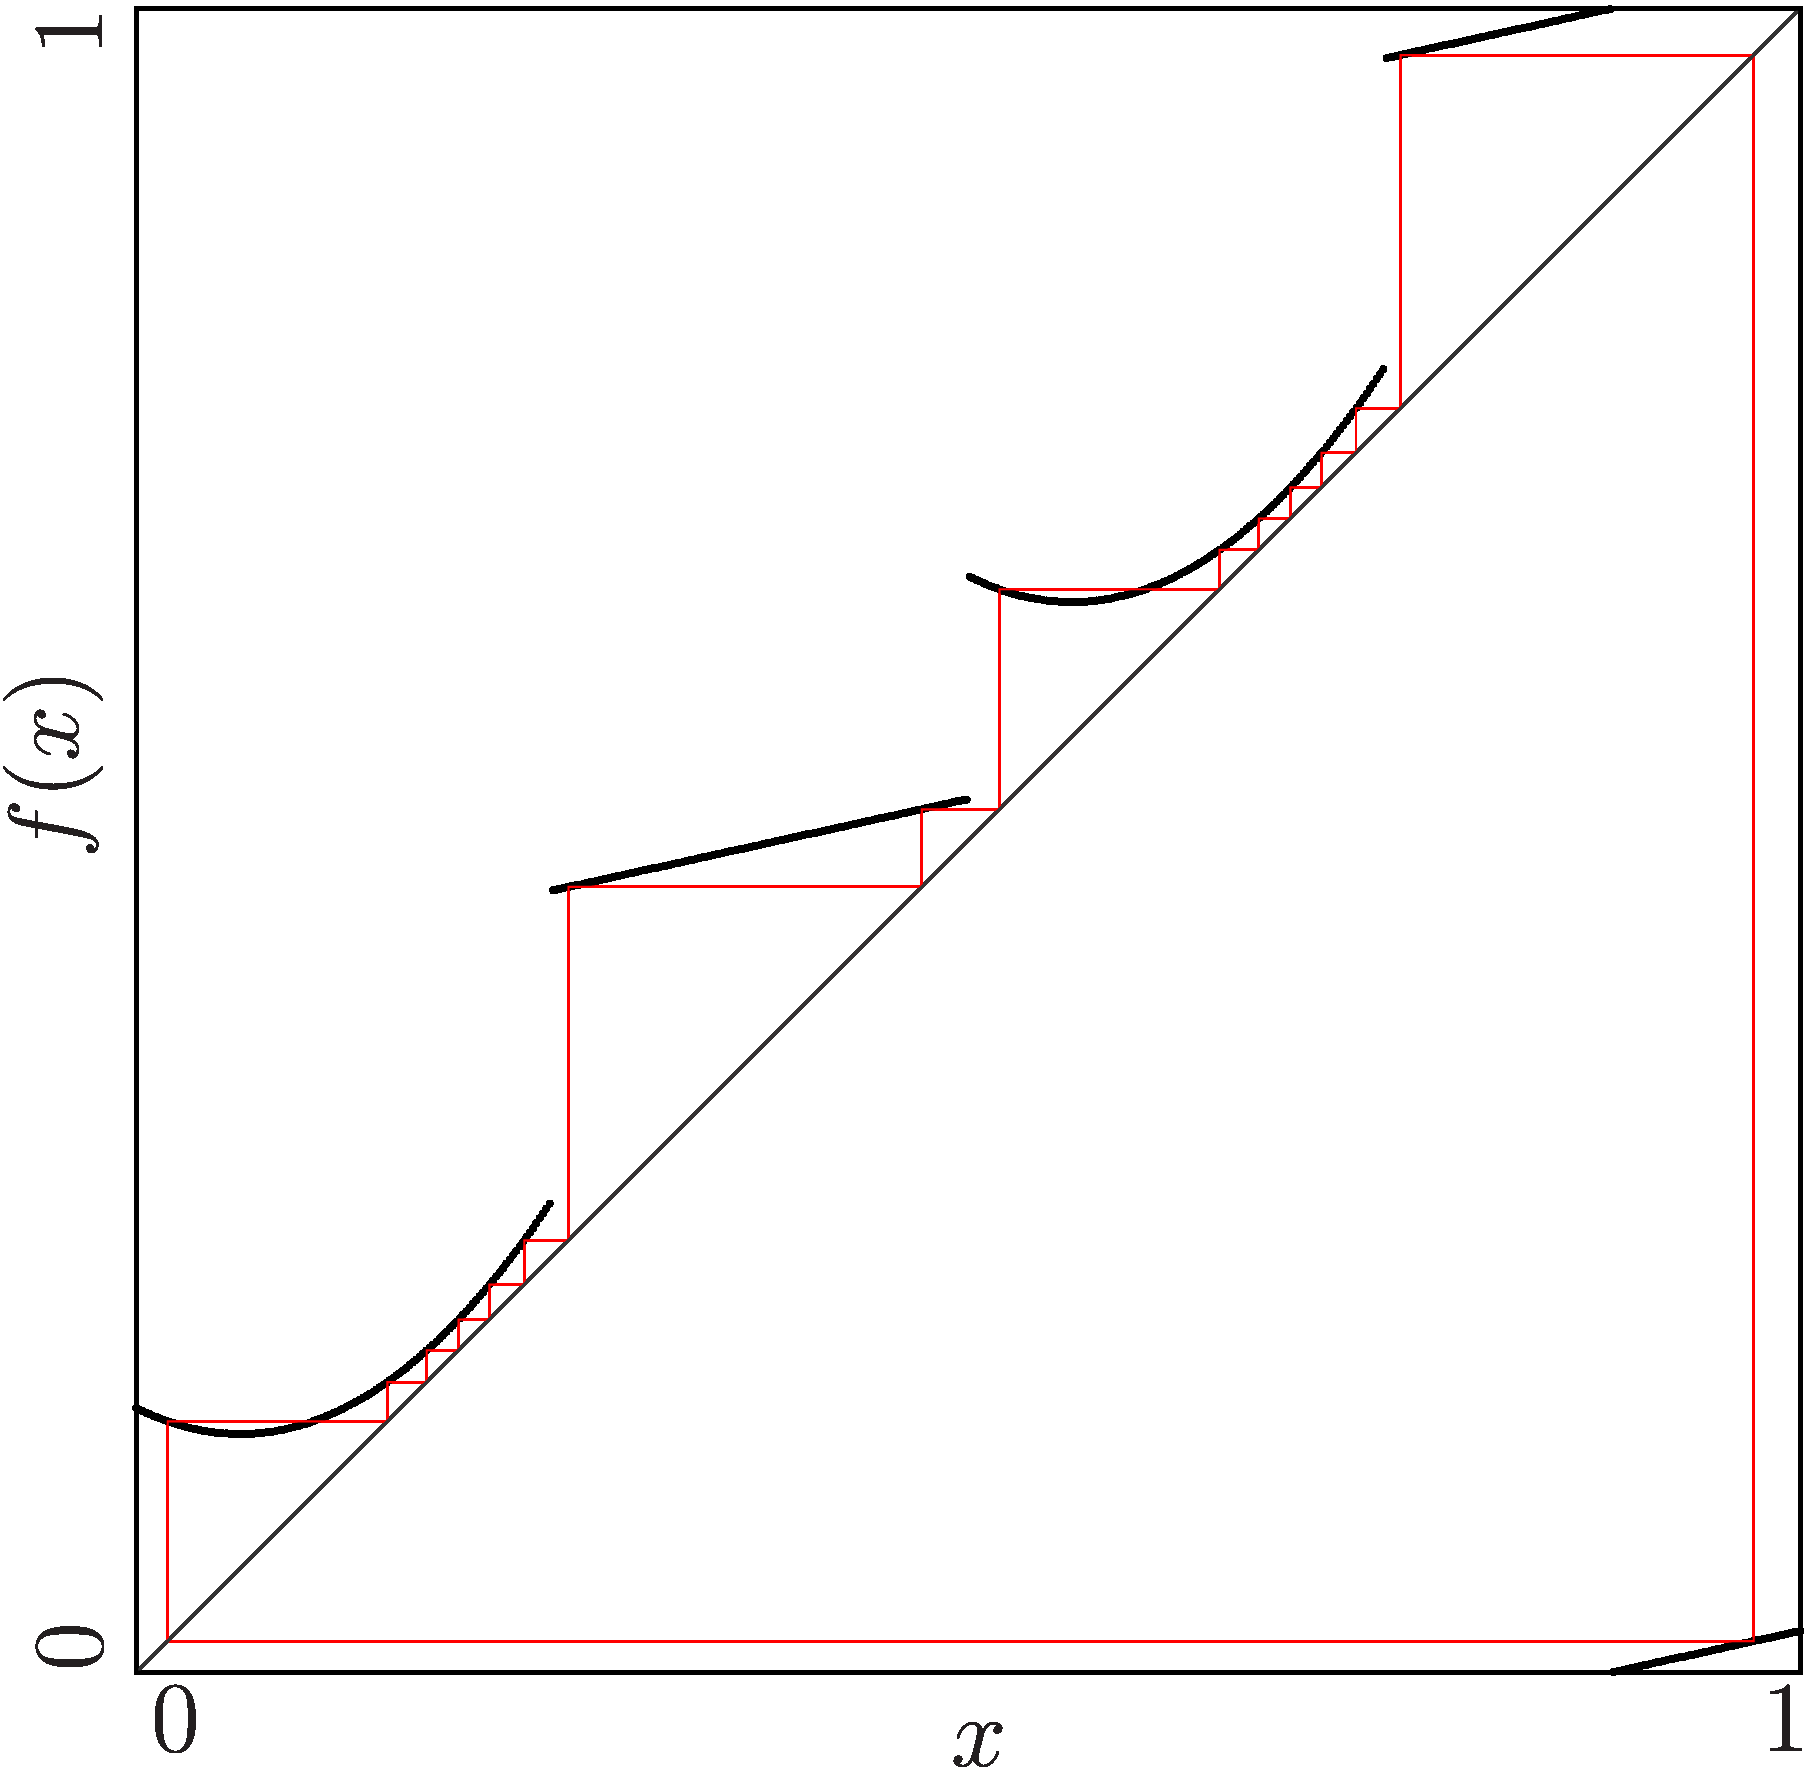
\includegraphics[width=0.3 \textwidth]{Figs/archetypal_model_cycle_c16.png}
        }{$C_{16}:\:\Cycle{\A^6\B^2\C^6\D^2}$}
        \stackunder[5pt]{
            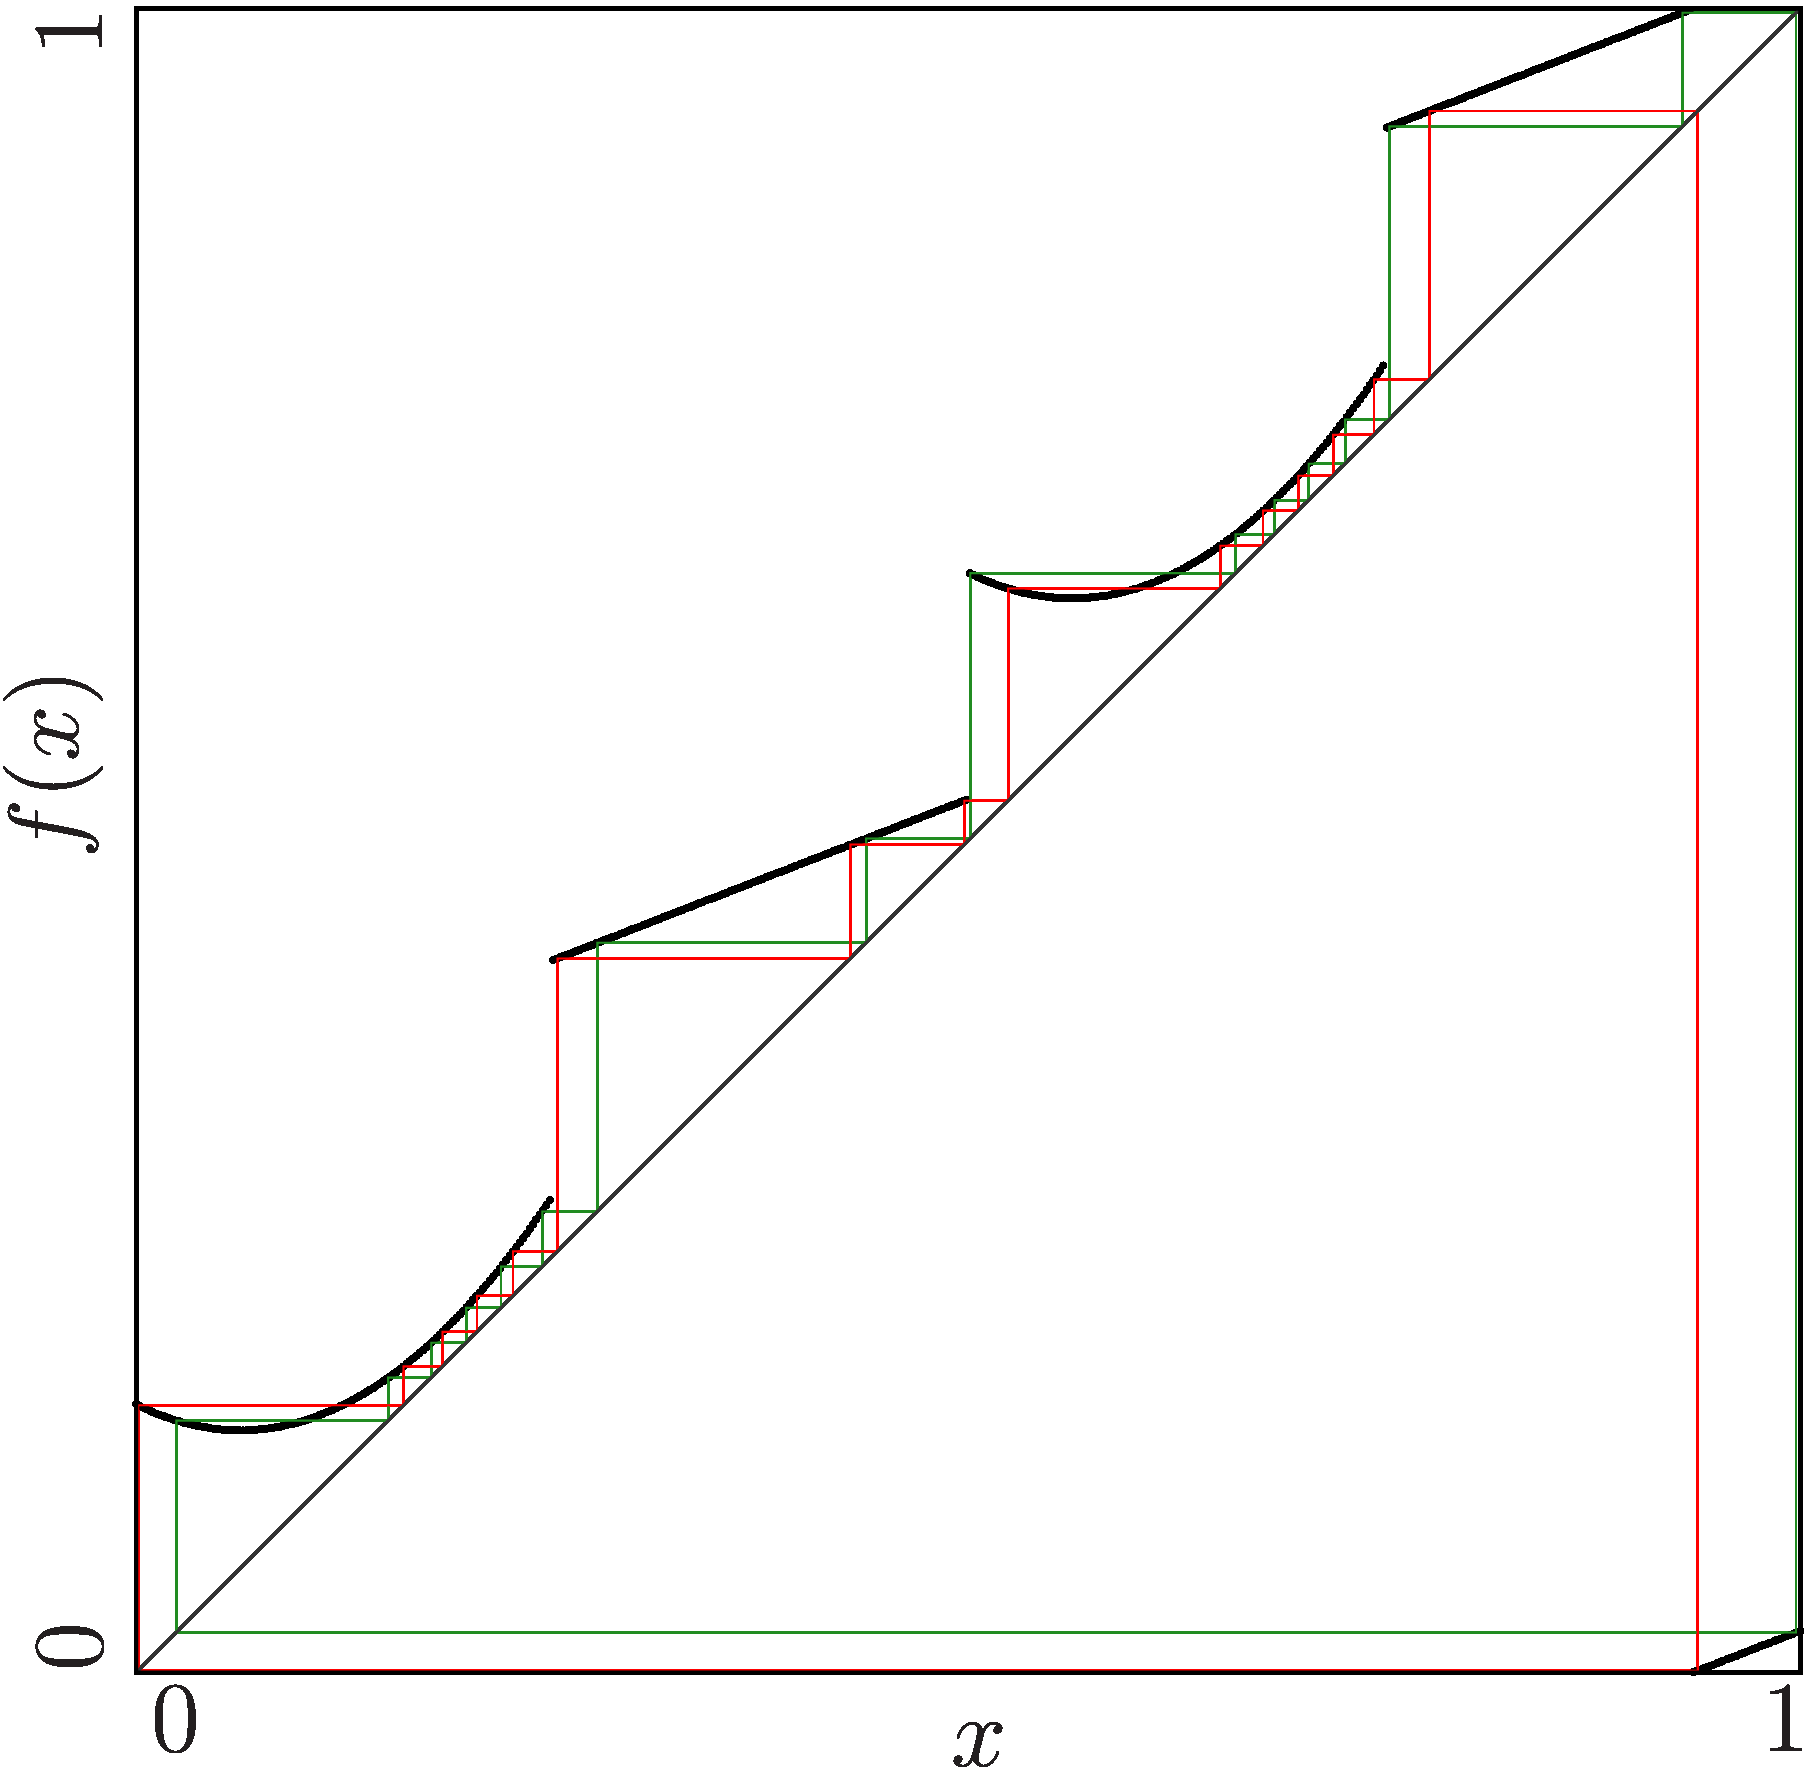
\includegraphics[width=0.3 \textwidth]{Figs/archetypal_model_cycle_d16.png}
        }{$D_{16}:\:\Cycle{\A^6\B^2\C^5\D^3},\Cycle{\A^5\B^3\C^6\D^2}$}
        \stackunder[5pt]{
            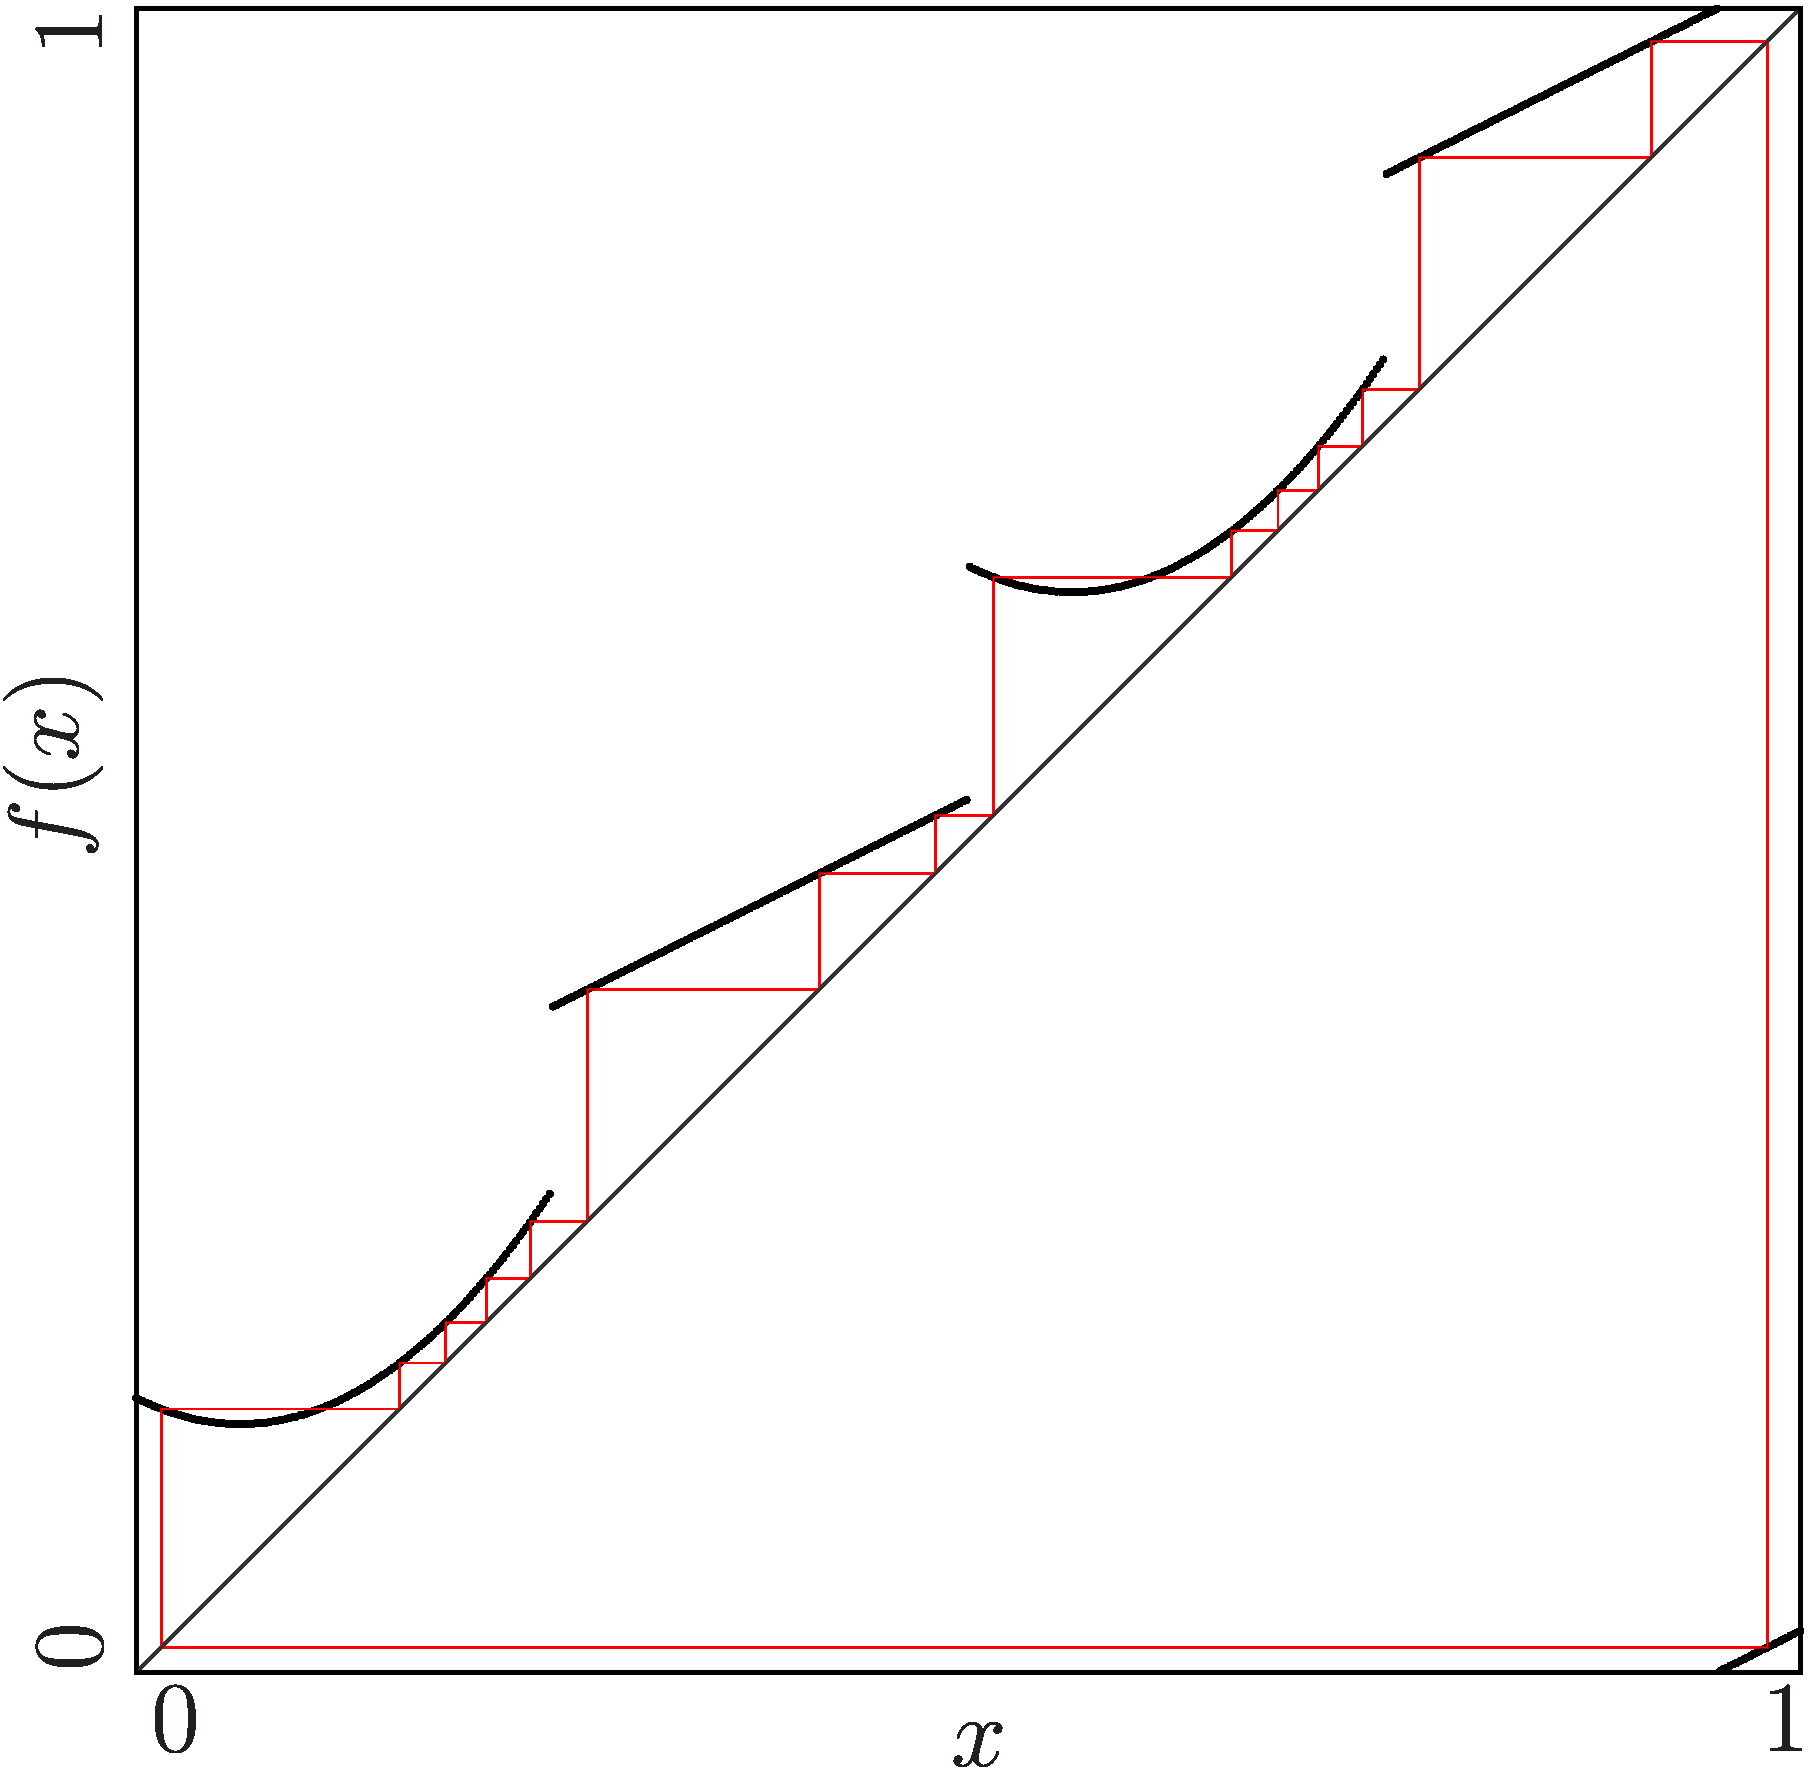
\includegraphics[width=0.3 \textwidth]{Figs/archetypal_model_cycle_e16.png}
        }{$E_{16}:\:\Cycle{\A^5\B^3\C^5\D^3}$}
    \end{figure}
\end{frame}

\begin{frame}{Archetypal Model Equations}
    \vspace{-1.0em}
    \begin{align*}
        x_{n+1} = f(x_n) \mod 1
    \end{align*}
    \begin{align*}
        f(x) & = \begin{cases}
                        g(x)                                        & \text{ if } x < \frac{1}{2} \\
                        g\left(x - \frac{1}{2}\right) + \frac{1}{2} & \text{ else}
                    \end{cases}
    \end{align*}
    \begin{align*}
        g(x) & = \begin{cases}
                        g_L(x) = a_L \cdot x^2 + b_L \cdot x + c_L & \text{ if } x < \frac{1}{4} \\
                        g_R(x) = b_R \cdot x + c_R                 & \text{ else}
                    \end{cases}
    \end{align*}
\end{frame}

\begin{frame}{Archetypal Model Equations}
    \vspace{-1em}
    \begin{columns}
        \begin{column}{.7 \textwidth}
            Fixed parameters:
            \begin{align*}
                a_L = 4 \text{ and } b_L = -\tfrac{1}{2}
            \end{align*}
            Variable parameters
            \begin{align*}
                    & c_L, b_R, c_R                                                                                                              \\
                \text{where} \qquad
                    & c_L = \beta,                                                                                                               \\
                    & b_R = -4 \cdot g_R\left(\tfrac{1}{4}\right) + 4 \cdot g_R\left(\tfrac{1}{2}\right),                                        \\
                    & c_R = 2 \cdot g_R\left(\tfrac{1}{4}\right) - 1 \cdot g_R\left(\tfrac{1}{2}\right),                                         \\[1em]
                \text{and} \qquad
                    & g_R\left(\tfrac{1}{4}\right) = \alpha, \text{and } g_R\left(\tfrac{1}{2}\right) = \tfrac{1}{2} + \epsilon \text{ is fixed}
            \end{align*}
        \end{column}
        \begin{column}{.3 \textwidth}
            \begin{figure}
                \centering
                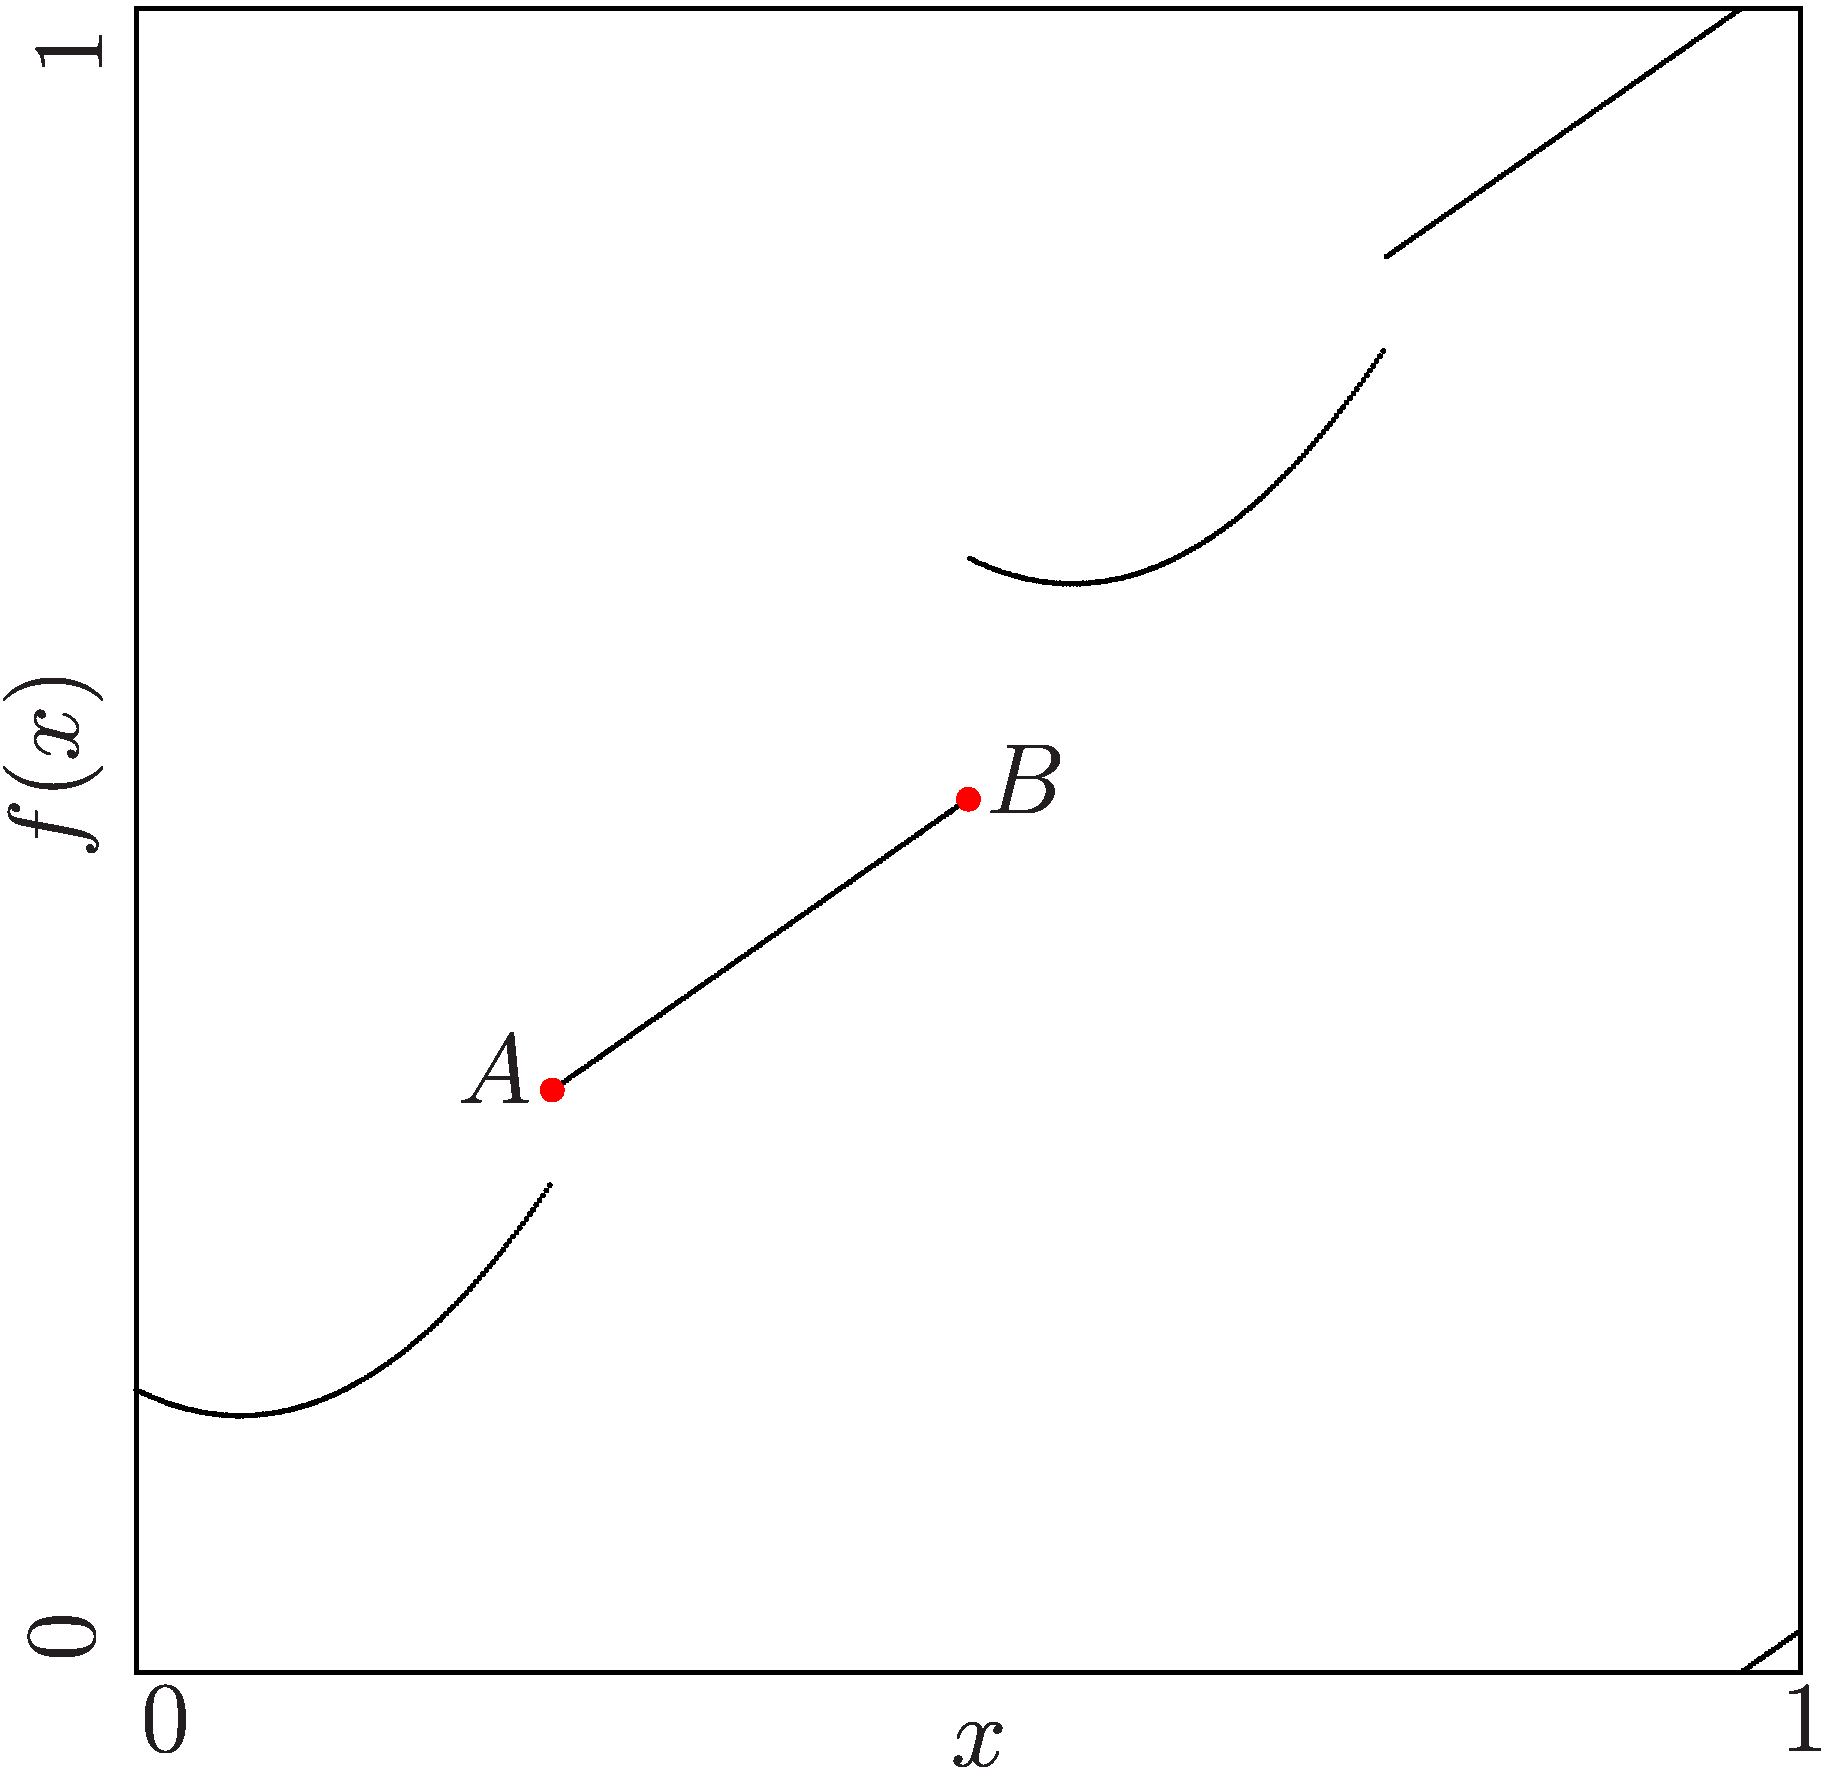
\includegraphics[height=.5 \textheight]{Figs/archetypal_model_parameter_effects_illustration.png}
            \end{figure}
        \end{column}
    \end{columns}
\end{frame}

%%% Local Variables:
%%% mode: latex
%%% TeX-master: "../Vortrag_Frauenhofer_Weik"
%%% End:
